\documentclass{article}
\usepackage[paperwidth=312mm,paperheight=105mm,margin=5mm]{geometry}
\usepackage{tikz}
\usepackage{amsmath}
\usepackage{sansmath}
\usetikzlibrary{arrows.meta,positioning,fit,calc}
\pagestyle{empty}
\setlength{\parindent}{0pt}
\begin{document}
\sffamily\sansmath
\centering
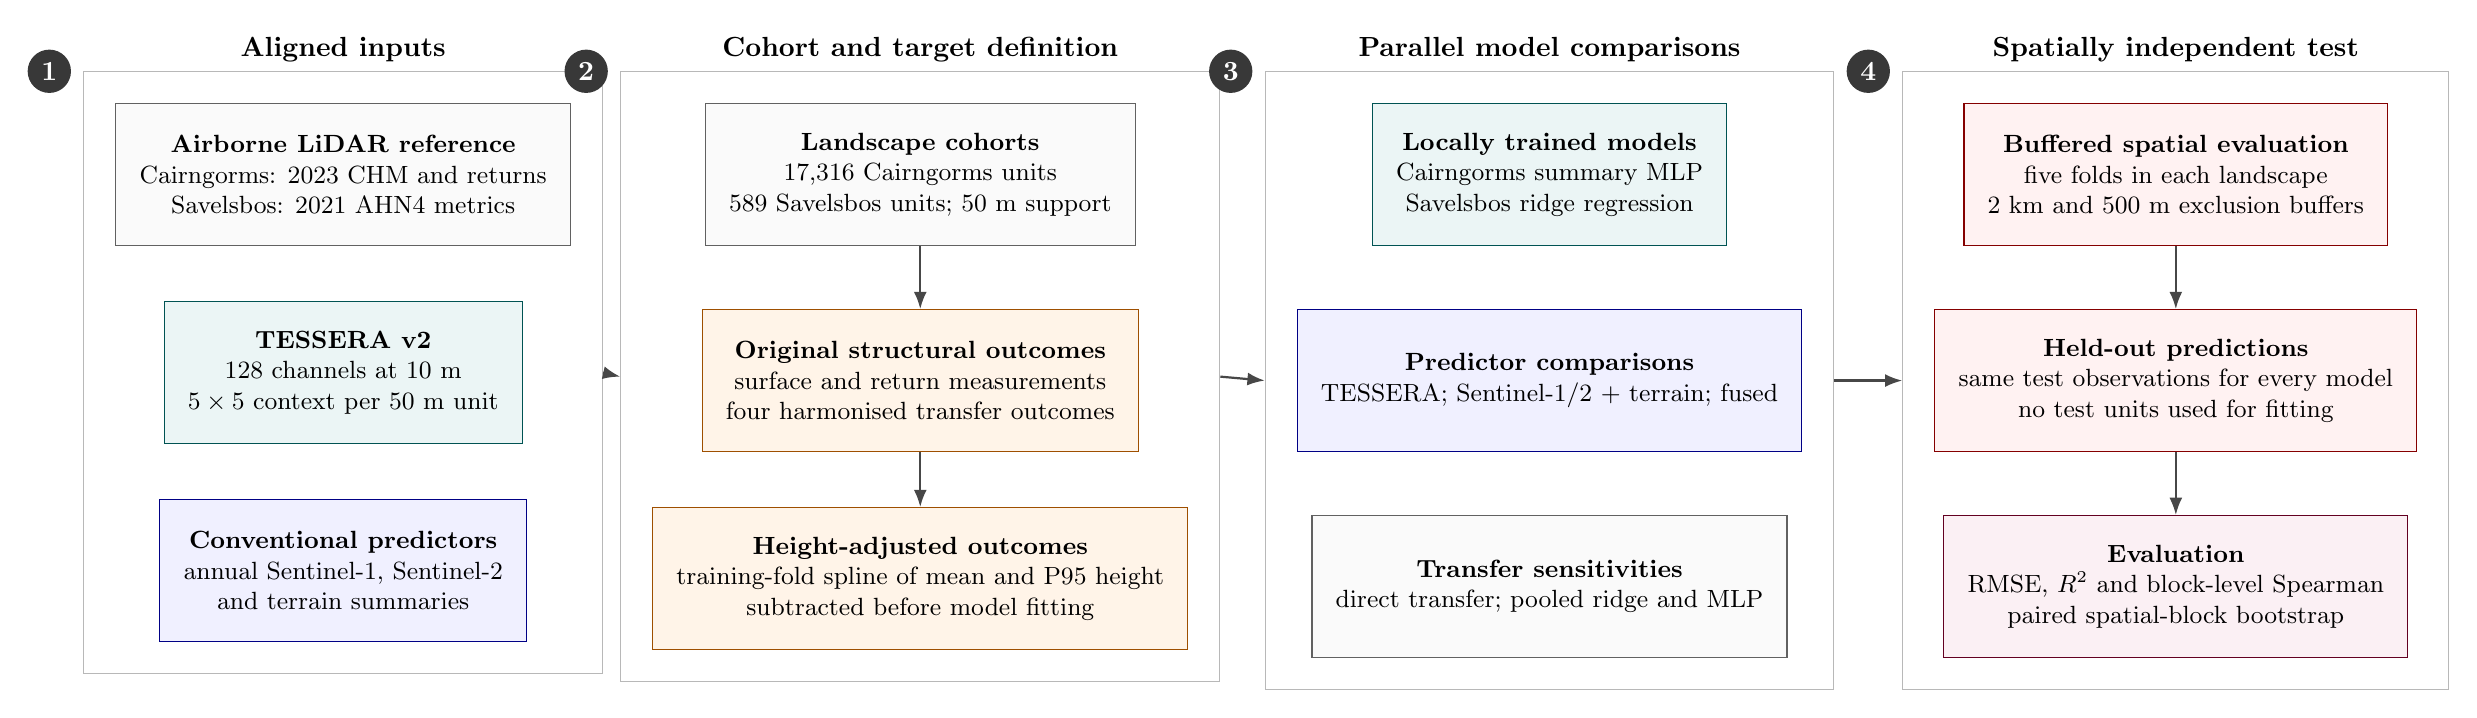
\begin{tikzpicture}[
  font=\small,
  >=Latex,
  arrow/.style={-{Latex[length=2.2mm]}, line width=0.8pt, draw=black!72},
  source/.style={draw=black!62, fill=black!2,
    minimum width=37mm, minimum height=18mm, align=center, inner sep=3mm},
  tessera/.style={source, draw=teal!65!black, fill=teal!8},
  conventional/.style={source, draw=blue!52!black, fill=blue!6},
  target/.style={source, draw=orange!62!black, fill=orange!9},
  evaluation/.style={source, draw=red!52!black, fill=red!5},
  result/.style={source, draw=purple!52!black, fill=purple!6},
  group/.style={draw=black!28, inner sep=4mm},
  stepbadge/.style={circle, fill=black!78, text=white, font=\bfseries,
    minimum size=5.5mm, inner sep=0pt}
]

\node[source] (lidar) {\textbf{Airborne LiDAR reference}\\
Cairngorms: 2023 CHM and returns\\
Savelsbos: 2021 AHN4 metrics};
\node[tessera, below=7mm of lidar] (tessera) {\textbf{TESSERA v2}\\
128 channels at 10 m\\
$5\times5$ context per 50 m unit};
\node[conventional, below=7mm of tessera] (conventional) {\textbf{Conventional predictors}\\
annual Sentinel-1, Sentinel-2\\
and terrain summaries};
\node[group, fit=(lidar)(conventional), label={[font=\bfseries]above:Aligned inputs}] (inputs) {};
\node[stepbadge, anchor=east] at ($(inputs.north west)+(-1.5mm,0)$) {1};

\node[source, right=17mm of lidar] (cohort) {\textbf{Landscape cohorts}\\
17,316 Cairngorms units\\
589 Savelsbos units; 50 m support};
\node[target, below=8mm of cohort] (raw) {\textbf{Original structural outcomes}\\
surface and return measurements\\
four harmonised transfer outcomes};
\node[target, below=7mm of raw] (adjusted) {\textbf{Height-adjusted outcomes}\\
training-fold spline of mean and P95 height\\
subtracted before model fitting};
\node[group, fit=(cohort)(raw)(adjusted), label={[font=\bfseries]above:Cohort and target definition}] (targets) {};
\node[stepbadge, anchor=east] at ($(targets.north west)+(-1.5mm,0)$) {2};

\node[tessera, right=30mm of cohort] (mlp) {\textbf{Locally trained models}\\
Cairngorms summary MLP\\Savelsbos ridge regression};
\node[conventional, below=8mm of mlp] (ridge) {\textbf{Predictor comparisons}\\
TESSERA; Sentinel-1/2 + terrain; fused};
\node[source, below=8mm of ridge] (fused) {\textbf{Transfer sensitivities}\\
direct transfer; pooled ridge and MLP};
\node[group, fit=(mlp)(ridge)(fused), label={[font=\bfseries]above:Parallel model comparisons}] (models) {};
\node[stepbadge, anchor=east] at ($(models.north west)+(-1.5mm,0)$) {3};

\node[evaluation, right=30mm of mlp] (folds) {\textbf{Buffered spatial evaluation}\\
five folds in each landscape\\
2 km and 500 m exclusion buffers};
\node[evaluation, below=8mm of folds] (predictions) {\textbf{Held-out predictions}\\
same test observations for every model\\
no test units used for fitting};
\node[result, below=8mm of predictions] (metrics) {\textbf{Evaluation}\\
RMSE, $R^2$ and block-level Spearman\\
paired spatial-block bootstrap};
\node[group, fit=(folds)(predictions)(metrics), label={[font=\bfseries]above:Spatially independent test}] (testing) {};
\node[stepbadge, anchor=east] at ($(testing.north west)+(-1.5mm,0)$) {4};

\draw[arrow] (inputs.east) -- (targets.west);
\draw[arrow] (cohort) -- (raw);
\draw[arrow] (raw) -- (adjusted);
\draw[arrow] (targets.east) -- (models.west);
\draw[arrow] (models.east) -- (testing.west);
\draw[arrow] (folds) -- (predictions);
\draw[arrow] (predictions) -- (metrics);

\end{tikzpicture}
\end{document}
